\section{Committing the witness}\label{sec:commit}

Only $\ff$ is committed. $\hh$ is derived and never appears here --- that is the
whole point of \cref{sec:arith}. The map is
\begin{equation}\label{eq:cw}
  \cw{\ff} \;\defeq\; \Enc_{\cC}\bigl(\pack(\pitwo(\bitsop(\ff)))\bigr)
  \;\in\;\comfield^{m},
  \qquad \orc \defeq \cw{\ff},
\end{equation}
and the prover publishes a Merkle root over $\orc$. Three objects appear in that
one line and keeping them apart makes the rest of the note readable: the
\emph{committed bits} $\ff\in\bits^{\ell}$, the \emph{packed vector}
$P\in\comfield^{\ell/128}$, and the \emph{codeword} $\orc$. (A polynomial
witness would need a fourth --- the bit vector $\bitsop(\ff)$ --- but here
$\bitsop$ is the identity.)

\subsection{From bits to a flat bit vector}

The witness is a bit vector, so there is nothing to decompose --- a SHA-256
\emph{word} is simply $32$ adjacent committed bits, and $\bitsop(\ff)=\ff$. What
remains is a layout question, and \emph{the order is load-bearing}, because $M$
is indexed by bit position and the code is indexed by lane.

\begin{center}
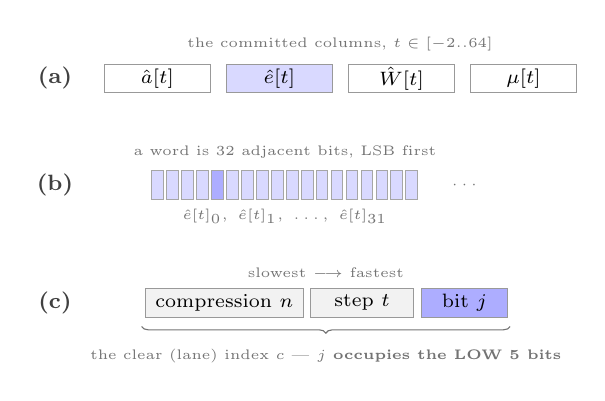
\begin{tikzpicture}[
  font=\scriptsize,
  cel/.style={draw=black!40, minimum width=0.62cm, minimum height=0.36cm,
              inner sep=0pt, line width=0.3pt},
  bitc/.style={draw=black!35, minimum width=0.15cm, minimum height=0.36cm,
              inner sep=0pt, line width=0.25pt},
  hlA/.style={fill=blue!15},
  hlB/.style={fill=blue!32},
  lbl/.style={font=\footnotesize\bfseries, text=black!75},
  dcap/.style={font=\tiny, text=black!55, align=center},
  arr/.style={-{Latex[length=1.8mm]}, draw=black!50, line width=0.5pt},
]
%% Three stacked rows with a left gutter for the panel letters.  A side-by-side
%% layout put the (b) and (c) labels on top of the arrow captions.
\def\GUT{-1.30}

%% ---- (a) the committed columns ----
\begin{scope}[shift={(0,0)}]
  \foreach \i/\lab in {0/{\hat a},1/{\hat e},2/{\hat W},3/{\mu}} {
    \pgfmathsetmacro\bx{\i*1.55}
    \ifnum\i=1
      \node[cel, hlA, minimum width=1.35cm] at (\bx,0) {$\lab[t]$};
    \else
      \node[cel, minimum width=1.35cm] at (\bx,0) {$\lab[t]$};
    \fi
  }
  \node[dcap] at (2.32,0.44) {the committed columns, $t\in[-2..64]$};
  \node[lbl]  at (\GUT,0) {(a)};
\end{scope}

%% ---- (b) one word expanded into its coefficients ----
\begin{scope}[shift={(0,-1.35)}]
  \foreach \k in {0,...,17} {
    \pgfmathsetmacro\bx{\k*0.19}
    \ifnum\k=4
      \node[bitc, hlB] at (\bx,0) {};
    \else
      \node[bitc, hlA] at (\bx,0) {};
    \fi
  }
  \node[dcap] at (3.90,0) {$\cdots$};
  \node[dcap] at (1.62,0.42) {a word is $32$ adjacent bits, LSB first};
  \node[dcap] at (1.62,-0.40) {$\hat e[t]_0,\ \hat e[t]_1,\ \dots,\ \hat e[t]_{31}$};
  \node[lbl]  at (\GUT,0) {(b)};
\end{scope}

%% ---- (c) the flat index ----
\begin{scope}[shift={(0,-2.85)}]
  \node[cel, minimum width=2.0cm, fill=black!5] at (0.85,0) {compression $n$};
  \node[cel, minimum width=1.3cm, fill=black!5] at (2.60,0) {step $t$};
  \node[cel, minimum width=1.1cm, hlB]          at (3.90,0) {bit $j$};
  \node[dcap] at (2.14,0.38) {slowest $\longrightarrow$ fastest};
  \draw[decorate, decoration={brace, amplitude=2.4pt, mirror}, draw=black!55]
    (-0.20,-0.30) -- (4.48,-0.30);
  \node[dcap] at (2.14,-0.68)
    {the clear (lane) index $c$ --- \textbf{$j$ occupies the LOW 5 bits}};
  \node[lbl]  at (\GUT,0) {(c)};
\end{scope}
\end{tikzpicture}
\captionof{figure}{Flattening. The bit position $j$ occupies the \emph{low}
five bits of the clear axis --- not a free choice; see
\cref{rem:layout}.}\label{fig:flatten}
\end{center}

\begin{remark}[Why $j$ must be lowest]\label{rem:layout}
The tap machinery that realises $M$ asserts $g\leq s$: the word group width
$g=5$ must fit inside the clear axis, because $\ROTR$ and $\SHR$ are
implemented as permutations of \emph{clear rows}
\src{src/taps.rs}. Word offsets need $\mathit{off}<2^{s-g}$, and the schedule
reads $\hat W[t{-}16]$, so $s\geq11$; containing a whole per-compression role
block wants $s\geq13$. This is the single layout pin the whole construction
hangs on, and it is the reason the alternative bit-diagonal virtualization path
cannot express SHA-256 at all.
\end{remark}

\subsection{The transpose}\label{sec:committedorder}

The flat order of \cref{fig:flatten} is \emph{not} the committed order. Between
the two sits the one genuine permutation on the entire commit path, and \S2.1's
claim that ``the order is load-bearing'' is really a claim about this step.

Write the flat index as $(\text{fold }b \mid \text{clear }c)$. The commitment
reads the bit matrix \emph{column by column}:
\[
  \underbrace{b\cdot 2^{s} + c}_{\text{flat}}
  \;\longmapsto\;
  \underbrace{c\cdot 2^{t_w} + b}_{\text{committed}},
  \qquad t_w \;=\; \text{row-bit width},
\]
a per-column gather with stride $2^{s}$ --- exactly the transpose of the
$2^{t}\times2^{s}$ bit matrix. \src{src/ligerito.rs}~\code{repack\_leaf\_bits},
target shape documented at \src{src/pcs.rs} as
$M[c][(b\ll\log_2 W)\,|\,j]$.

\begin{warning}[Two readings of \cref{fig:flatten} do not survive it]
\label{warn:transpose}
\Cref{fig:flatten}(b) says ``a word is $32$ adjacent bits''. That is true of the
\emph{flat} order and false of the committed one: after the transpose the $32$
bits of one SHA-256 word differ only in the clear index, so they are strided by
$2^{t_w}$.

The consequence lands on the next figure. A $128$-bit pack window contains
\textbf{at most one bit of any SHA-256 word} --- it is one fixed clear slot read
across $128$ consecutive fold rows, not four adjacent words. A reader who
carries the flat picture forward will conclude that a packed
$\comfield$ element holds four words of the trace. It holds one bit from each of
$128$ different rows.
\end{warning}

\noindent
With that named, the rest of the path is easy to state, because \emph{nothing
else moves}:

\begin{center}\small
\begin{tabular}{@{}llp{0.46\textwidth}@{}}
\toprule
step & moves? & what it is\\
\midrule
transpose      & \textbf{yes} & per-column gather, stride $2^{s}$
                 --- \code{repack\_leaf\_bits}\\
pack to $\comfield$ & no & blocking of a contiguous array\\
interleave     & no & index decomposition; the SoA order already matches\\
rate expansion & no & contiguous replication of the message\\
RS encode      & no & arithmetic in place, lane-wise (additive NTT)\\
\bottomrule
\end{tabular}
\end{center}

\noindent
So the answer to ``where does the reordering happen?'' is: once, here, and never
again. Everything after this line is the same bits in the same order, viewed
through different index decompositions.

\begin{warning}[Which commit path a SHA-256 instance takes is not pinned]
\label{warn:twopaths}
The repository carries \emph{two} layouts --- one placing the bit position on the
fold axis, one on the clear axis with $g=5$ (\cref{rem:layout} describes the
latter) --- and the transpose above belongs to the first. The second commits
packed clear rows directly. Neither builder has a call site under
\code{src/}, \code{examples/}, \code{benches/} or \code{tests/}, and no test
pins the packed-message index map; correctness is enforced only indirectly, by a
ring-switch recombination assertion and end-to-end round trips. So the layout
this section prints is the documented one, not a measured one. A direct test of
the index map would be cheap insurance.
\end{warning}

\subsection{The two axes, and who fixes them}\label{sec:axes}

The transpose above is what splits the witness into a matrix, and that matrix's
shape is a \emph{commitment-time} decision --- fixed by
\code{IntEvalParams}$\{t,s,\text{word\_bits}\}$ before anything is proved. Write
\[
  \begin{gathered}
    \ell = \ellrow\ellcol,\\
    \ellrow = 2^{t_w}\; (\text{row/fold axis}),
    \qquad
    \ellcol = 2^s\; (\text{column/clear axis}).
  \end{gathered}
\]
These are the paper's $\ell_1$ and $\ell_2$, respectively; semantic names are
used from here on. Here $t_w=t+\log_2 W$ --- \code{row\_bit\_vars}, \emph{not} the struct field
\code{ShaF2Layout.tw}, which is a different and smaller quantity ($6$ against
$t=13$ at one shipped layout, so $2^{\mathtt{tw}}=64$ where $\ellrow=8192$). Everything downstream inherits this and nothing
downstream can change it: $\ellrow$ is the number of rows in each grand product in
\cref{step:gkr}, and $\ellcol$ is the number of column integers the prover puts in the
clear at \cref{step:tensor}.

What makes the choice interesting is that \textbf{three unrelated layers each
pin one end of it}, and they very nearly meet:

\begin{center}\small
\begin{tabular}{@{}llp{0.40\textwidth}@{}}
\toprule
bound & from & why\\
\midrule
$t_w\geq7$        & the pack & a $\comfield$ element is $128$ bits, so
                                $128\mid\ellrow$ \src{src/ligerito\_flock.rs}\\
$s\geq13$         & the taps & rotations are permutations of clear rows and
                                need $g\leq s$; a whole per-compression role
                                block wants $s\geq13$ (\cref{rem:layout})\\
$t+W\leq127-q_{\text{bits}}$ & \textbf{the exponent fold}
                  & the honest column sum must not wrap $\ord(g)$; for a
                    $100$-bit prime this is $t+W<28$ \src{src/pcs.rs}\\
\bottomrule
\end{tabular}
\end{center}

\noindent
The third is the one to notice, and it is easy to overstate. It is a
\textbf{soundness} bound arriving from four steps away, so the commitment layout
and the exponent fold of \cref{step:exponent} are not independent choices ---
something neither section says on its own. But it is a \emph{ceiling}, not a
forcing constraint: unsplit ($\ellcol=1$) the single exponent first wraps at
$\ell=2^{29}$, and limb chunking pushes even that to $\ell\approx2^{125}$ at a
cost of $L=\lceil q_{\text{bits}}/c_w\rceil$ parallel forests. The paper
explicitly admits the trivial decomposition $\ellrow=\ell$, $\ellcol=1$.

\textbf{So why split at all? Verifier cost.} The verifier's only
super-logarithmic work is one $\Theta(\ellrow)$ pass --- $2^{t}$ wide fixed-base
exponentiations building the weight table \src{row\_bit\_weights --- src/pcs.rs}
--- and one $\Theta(\ellcol)$ pass over the sent integers. Unsplit that is
$\Theta(\ell)$: a full witness-length sweep, and no succinctness at all. Split,
it is $\Theta(\ellrow+\ellcol)$, minimised near $\sqrt\ell$. Chunking cannot
substitute, because it \emph{multiplies} the verifier by $L$.

Where the shape shows up in cost, then: $\ellcol$ drives \emph{proof size} ---
$L\cdot\ellcol$ integers of $16$ bytes each, about $43\%$ of the whole proof at
$n=26$, $s=13$ --- so a larger $\ellrow$ shrinks the proof. \emph{Prover} time is
$\Theta(\ellrow\ellcol)=\Theta(\ell)$ whichever way the split falls; the forest
evaluates every leaf and every internal node regardless (\cref{step:gkr}).
Every layout in the repository makes $s$ a fixed fraction of $n$ ($\lfloor
2n/5\rfloor$, or $\approx n/2$), so the sent-integer block is
$\Theta(N^{2/5})$--$\Theta(N^{1/2})$: neither constant nor linear in the number
of hashes. \Cref{sec:config} carries the measured numbers.

\subsection{From bits to a root}

\begin{center}
\begin{tikzpicture}[
  font=\scriptsize,
  bitc/.style={draw=black!35, minimum width=0.14cm, minimum height=0.34cm,
              inner sep=0pt, line width=0.25pt},
  fe/.style={draw=black!45, rounded corners=1pt, minimum width=0.88cm,
             minimum height=0.44cm, inner sep=0pt, line width=0.4pt},
  hlO/.style={fill=orange!40},
  hlOl/.style={fill=orange!15},
  lbl/.style={font=\footnotesize\bfseries, text=black!75},
  dcap/.style={font=\tiny, text=black!55, align=center},
  arr/.style={-{Latex[length=1.8mm]}, draw=black!50, line width=0.5pt},
  mk/.style={draw=black!45, circle, minimum size=0.24cm, inner sep=0pt,
             line width=0.35pt},
]
\def\GUT{-1.45}

%% ---- (a) pack ----
\begin{scope}[shift={(0,0)}]
  \foreach \k in {0,...,15} {
    \pgfmathsetmacro\bx{\k*0.14}
    \ifnum\k<5   \node[bitc, hlOl] at (\bx,0) {}; \fi
    \ifnum\k>4 \ifnum\k<11 \node[bitc, hlO] at (\bx,0) {}; \fi\fi
    \ifnum\k>10  \node[bitc, hlOl] at (\bx,0) {}; \fi
  }
  \draw[decorate, decoration={brace, amplitude=2.2pt}, draw=black!60]
    (5*0.14-0.07,0.26) -- (10*0.14+0.07,0.26);
  \node[dcap] at (1.05,0.58) {$128$ consecutive \emph{committed} bits};
  \node[dcap] at (1.05,-0.42) {$\pitwo(\bitsop(\ff))$};
  \node[lbl]  at (\GUT,0) {(a)};

  \draw[arr] (2.45,0) -- node[dcap, above, yshift=1pt]{$\pack$} (3.25,0);

  \node[fe, hlOl] at (3.72,0) {$P_1$};
  \node[fe, hlO]  at (4.66,0) {$P_2$};
  \node[fe, hlOl] at (5.60,0) {$P_3$};
  \node[dcap]     at (6.30,0) {$\cdots$};
  \node[fe, hlOl] at (7.05,0) {$P_{\ell/128}$};
  \node[dcap] at (5.38,-0.44) {$P\in\comfield^{\ell/128}$, \code{LOG\_PACKING}$=7$};
\end{scope}

%% ---- (b) interleave + encode --- POSITION-MAJOR.
%% flock stores codeword[pos * num_ntts + lane]: rows = code positions (a row is
%% one contiguous Merkle leaf), columns = lanes (a column is one RS codeword).
%% The encoder runs DOWN a column; expansion ADDS ROWS.  The earlier drawing had
%% this transposed, which made the leaf a gather -- the thing flock avoids.
%% Every annotation sits OUTSIDE both blocks; labels beside the cells overlapped
%% them, and the log says nothing about that.
\begin{scope}[shift={(0,-2.45)}]
  \foreach \r in {0,1,2} {
    \pgfmathsetmacro\yy{-\r*0.40}
    \foreach \c in {0,1,2,3} {
      \pgfmathsetmacro\bx{\c*0.46}
      \ifnum\r=0 \ifnum\c=1 \node[fe, hlO, minimum width=0.38cm] at (\bx,\yy) {};
        \else \node[fe, hlOl, minimum width=0.38cm] at (\bx,\yy) {}; \fi
      \else \node[fe, hlOl, minimum width=0.38cm] at (\bx,\yy) {}; \fi
    }
  }
  \node[dcap] at (0.69,0.52) {message\\$2^{m_p-k_0}$ positions};
  \draw[arr] (1.95,-0.40) -- (2.60,-0.40);

  \foreach \r in {0,...,5} {
    \pgfmathsetmacro\yy{-\r*0.40}
    \foreach \c in {0,1,2,3} {
      \pgfmathsetmacro\bx{3.05+\c*0.46}
      \ifnum\c=1
        \ifnum\r=0 \node[fe, hlO,  minimum width=0.38cm] at (\bx,\yy) {};
        \else      \node[fe, hlOl, minimum width=0.38cm] at (\bx,\yy) {}; \fi
      \else \node[fe, minimum width=0.38cm, fill=black!5] at (\bx,\yy) {}; \fi
    }
  }
  \node[dcap] at (3.74,0.52) {codeword\\$2^{k_{\mathrm{code}}}$ positions};

  \draw[draw=black!70, line width=0.6pt, rounded corners=1pt]
    (3.05-0.26,-1.20+0.26) rectangle (3.05+3*0.46+0.26,-1.20-0.26);


  \draw[arr] (5.05,0.10) -- (5.05,-2.10);
  \node[dcap, anchor=west] at (5.18,-1.00)
    {additive NTT\\runs \emph{down}\\each lane};

  \node[dcap] at (2.60,-2.62)
    {$2^{k_0}$ lanes, each an independent RS codeword
     ($k_0=\code{initial\_k}$; $16$ by default);\\
     the outlined row is one Merkle leaf --- contiguous in memory};
  \node[lbl]  at (\GUT,-0.40) {(b)};
\end{scope}

%% ---- (c) Merkle ----
\begin{scope}[shift={(2.75,-6.30)}]
  \draw[draw=black!30, line width=0.4pt]
    (0.9,0.30) -- (0.45,-0.10) (0.9,0.30) -- (1.35,-0.10)
    (0.45,-0.10) -- (0.20,-0.52) (0.45,-0.10) -- (0.70,-0.52)
    (1.35,-0.10) -- (1.10,-0.52) (1.35,-0.10) -- (1.60,-0.52);
  \node[mk, fill=green!22] at (0.9,0.30) {};
  \node[mk] at (0.45,-0.10) {}; \node[mk] at (1.35,-0.10) {};
  \node[mk] at (0.20,-0.52) {}; \node[mk] at (0.70,-0.52) {};
  \node[mk] at (1.10,-0.52) {}; \node[mk] at (1.60,-0.52) {};
  \node[dcap] at (0.9,-0.94) {$\mathsf{root}$ (SHA-256); leaf $=$ one row,
     $2^{k_0}$ elements $=2^{k_0}{\cdot}16$ bytes};
  \node[lbl] at (\GUT-2.75,-0.10) {(c)};
\end{scope}
\draw[arr] (3.65,-5.35) -- (3.65,-5.87);
\end{tikzpicture}
\captionof{figure}{Packing, encoding and the root. Orange traces one $128$-bit
window becoming one $\comfield$ element, taking one slot of the message matrix,
and being spread by the encoder \emph{down} its lane. The matrix is drawn
position-major because that is how it is stored: a Merkle leaf is a contiguous
row, and no gather is ever performed.}\label{fig:toroot}
\end{center}

\begin{remark}[The witness does not become one big number]
``Pack the witness into $\comfield$'' invites the wrong picture. Each
\emph{consecutive block of $128$ bits} becomes one field element, so the result
is a \emph{vector} of $\ell/128$ elements; $128$ is a property of the
commitment field, not of the data. And packing never crosses a \emph{column}
boundary, because $128\mid\ellrow$ --- \src{src/ligerito\_flock.rs} asserts
$t+\log_2 W\geq7$. Lanes are a different axis entirely (\cref{warn:lanes}), and
the pack never has to know about them.
\end{remark}

\begin{warning}[A lane is not a compression, and $\ellcol$ is not $N$]
\label{warn:lanes}
Two shape claims that earlier drafts of this section carried are wrong, and both
matter downstream.

\textbf{The lane count is an encoder knob, not the trace.} Interleaving is
$2^{k_0}$-fold with $k_0=\code{initial\_k}$ --- $16$ lanes by default --- and the
lane index is the \emph{low} $k_0$ bits of the packed index, i.e.\ fold-side
coordinates sitting just above the seven the pack absorbed. So a lane is not
``one compression'', and every lane draws entries from every clear column.

\textbf{And $\ellcol$ is the clear-column count $2^{s}$, not $N$.} The
$\mu[\colidx]$ values of \cref{sec:iopp} are one per clear column, and each
grand product runs down the row/fold axis $\ellrow=2^{t_w}$. Mind what this does
and does not say: $\ell=\ellrow\ellcol$ is the \emph{total} committed bit count
and is $\Theta(N)$; only the $\ellcol$ factor is sublinear.  The sent-integer
block must therefore be costed against $2^s$, not against $N$.

Both statements are read off the configuration and commit code rather than
measured, and \cref{warn:twopaths} applies.
\end{warning}

\subsection{Where bit-ness comes from}

\Cref{warn:bitness} asked at which layer the $\bits$ guarantee enters. It enters
\emph{here}, and it is worth being precise because the whole arithmetization
leans on it.

$\pitwo:\Z\to\Ftwo$ is catastrophically lossy on a general integer --- that is
parity collapse, the obstruction F2Z exists to solve. On $\bits$ it is a
\emph{bijection}. So bit-decomposition is not a storage convention: it is the
precondition that makes the one unavoidable $\Z\to\Ftwo$ crossing
information-preserving. A cell of $\ff$ is a bit because the committed object
\emph{is} a bit vector --- there is no representation in which it could be
anything else.

The same restriction buys the exponent fold of \cref{sec:iopp}: $P(Y,Z)=(Y-1)Z+1$
is affine in $Z$ only because $Z\in\bits$.

\begin{remark}[What the root does \emph{not} bind]
The root binds $P$, hence $\bitsop(\ff)$, hence $\ff$ --- \emph{but only given
that $\orc$ is a codeword}, which nothing so far establishes. A cheating prover
can publish a root over an arbitrary vector. All binding is conditional on the
proximity test in \cref{step:proximity}, which is why the commitment claim stays
open in the ledger for the entire protocol rather than being discharged at
commit time.
\end{remark}
